    \begin{wrapfigure}[10]{l}{0.38\textwidth}
    \vspace{-3mm}
    \includegraphics[trim = 0mm 0mm -1mm 0mm, clip, width=0.38\textwidth]{images/lh03705_009r-d1.pdf}\\
\noindent \centering [\textit{Fig. 9}] 
    % \caption{Bildbeschreibung}
    \end{wrapfigure}
%[9~r\textsuperscript{o}]
Caeterum non rebus tantum per planum trahendis, sed et aliis corporibus in aliis innitentibus, et relictis illis movendis, nocet attritus\protect\index{Sachverzeichnis}{attritus}, ut funibus\protect\index{Sachverzeichnis}{funis} replicatis, quibus motus varie reguntur, huic rei remedium inventum est; pone a pondere \textit{A} attrahi pondus\protect\index{Sachverzeichnis}{pondus} \textit{B}, funem\protect\index{Sachverzeichnis}{funis} autem per trochleas\protect\index{Sachverzeichnis}{trochlea} \textit{C}. \textit{D} ire. Ponantur primum trochleae\protect\index{Sachverzeichnis}{trochlea} immobiles et in centris suis fixae, patet attritum\protect\index{Sachverzeichnis}{attritus} funis\protect\index{Sachverzeichnis}{funis} fore, contra trochleas\protect\index{Sachverzeichnis}{trochlea} in attactuum locis. At si mobiles sint trochleae\protect\index{Sachverzeichnis}{trochlea} patet idem fieri quod in rotis, ut vis movens\protect\index{Sachverzeichnis}{vis movens} rotam \edtext{agat radio}{\lemma{agat}\Bfootnote{\textit{(1)}\ centro \textit{(2)}\ radio \textit{L}}} \textit{EF}, unde et facile superatur attritus\protect\index{Sachverzeichnis}{attritus} qui restat in ipso \textit{E}, rotae contra axem, non tantum, quod exiguus esse potest, et quod potest ungi, hoc enim idem quodammodo praestari posset in loco attactus, \textit{F}, sed quod vis movens\protect\index{Sachverzeichnis}{vis movens} distantia a centro multiplicatur, unde \edtext{quanto trochlea major,}{\lemma{quanto}\Bfootnote{\textit{(1)}\ vis movens\protect\index{Sachverzeichnis}{vis movens} major, \textit{(2)}\ trochlea major, \textit{L}}} et circulus exiguus \textit{E}, vel attactus axis et trochleae\protect\index{Sachverzeichnis}{trochlea} minor, tanto facilior motus. Verum est a trochleae\protect\index{Sachverzeichnis}{trochlea} magnitudine aliud oriri incommodum, \edtext{nam circuli circumferentia magis}{\lemma{nam}\Bfootnote{\textit{(1)}\ circulus \textit{(2)}\ circuli circumferentia magis \textit{L}}} \edtext{accedit rectae}{\lemma{accedit}\Bfootnote{\textit{(1)}\ plano \textit{(2)}\ rectae, \textit{L}}}, ac proinde attritus\protect\index{Sachverzeichnis}{attritus} major, \edtext{sed ea}{\lemma{sed}\Bfootnote{\textit{(1)}\ id \textit{(2)}\ ea \textit{L}}} incommoditas, compensatur vi aucta, cum attritus\protect\index{Sachverzeichnis}{attritus} qui superest sit exiguus. 
\pend
\pstart
%    \begin{wrapfigure}{l}{0.33\textwidth}
%   \vspace{-10pt}
%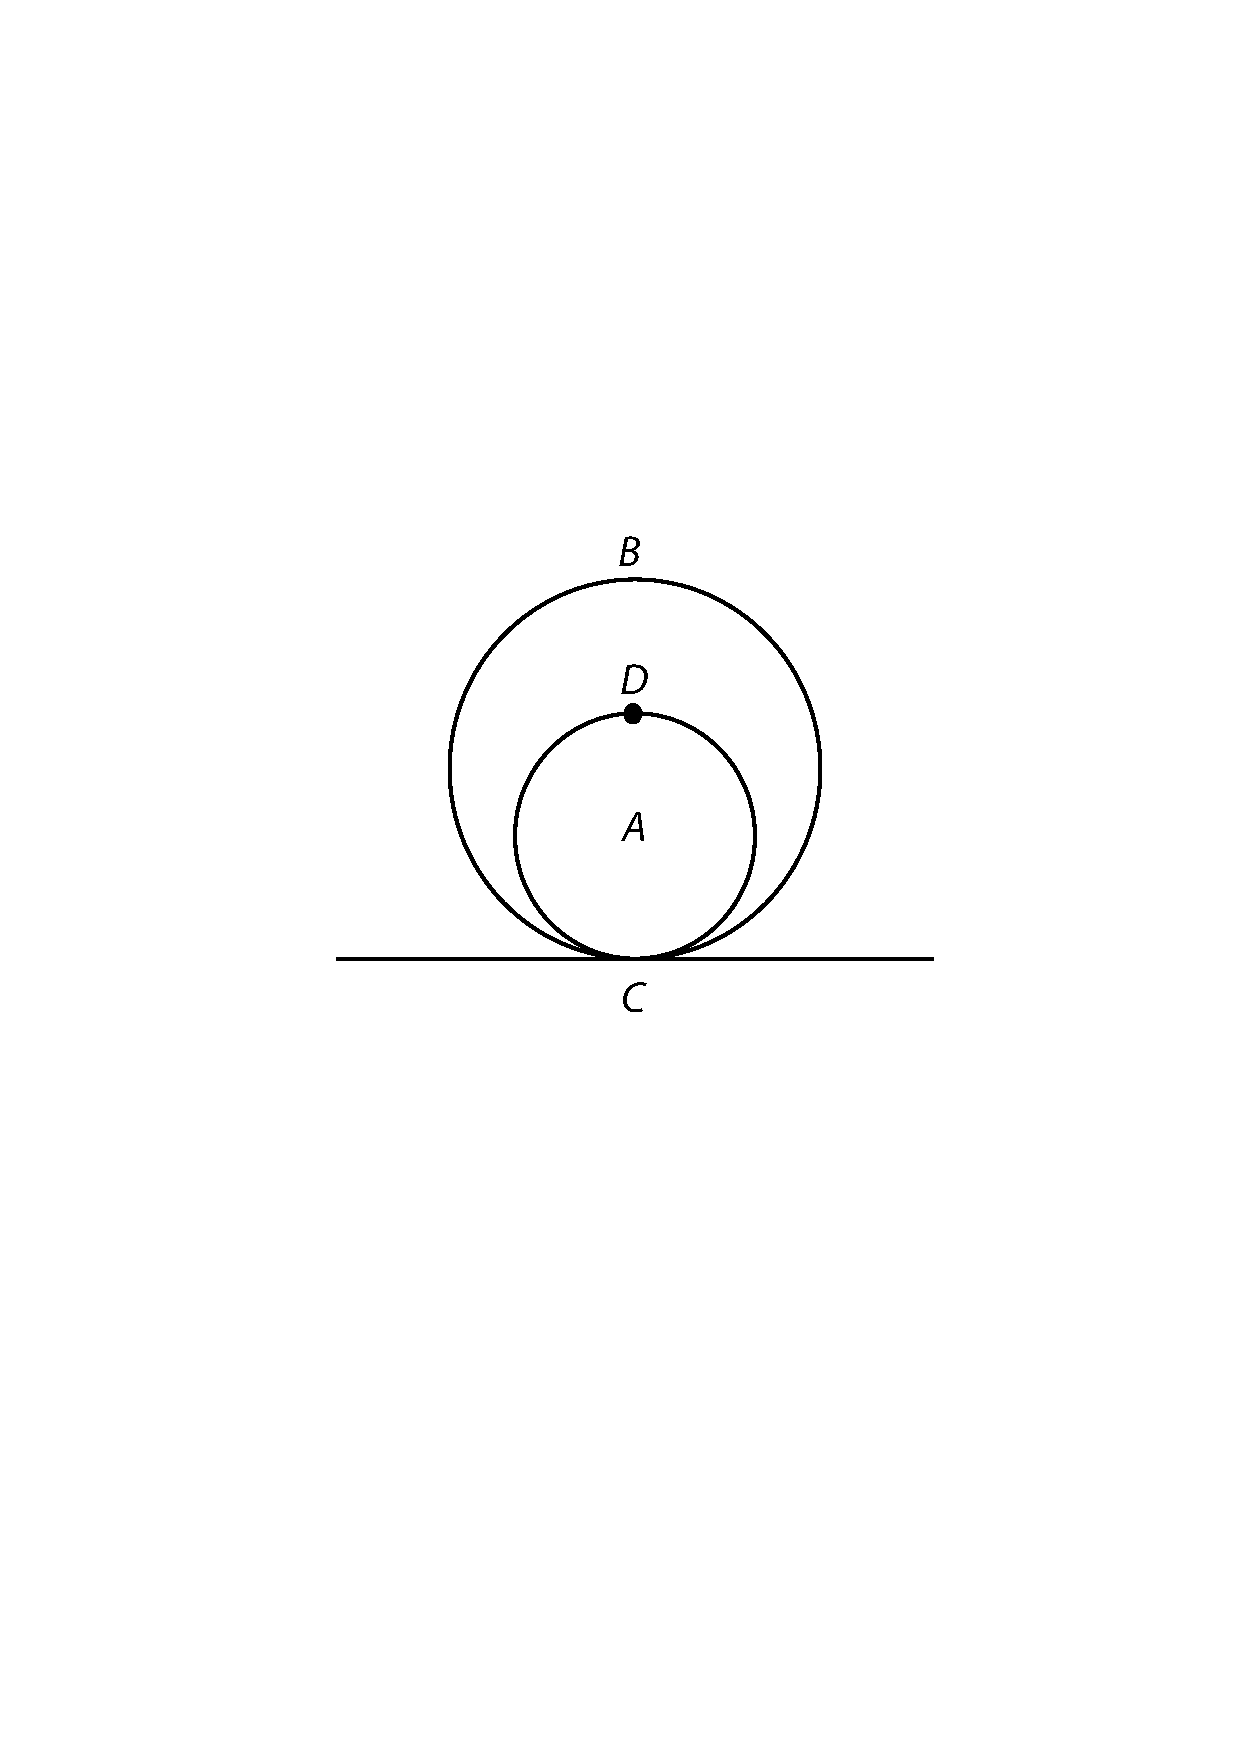
\includegraphics[trim = 58mm 125mm 45mm 90mm, clip, width=0.33\textwidth]{images/lh03705_009r-d2.pdf}
%    % \caption{Bildbeschreibung}
%\noindent \centering [\textit{Fig. 10}] 
%    \end{wrapfigure}
Esto circulus \textit{A} in circulo \textit{B}, quem intus \edtext{tangit circulus, \textit{A},}{\lemma{}\Bfootnote{tangit \textbar\ circulus \textit{erg.} \textbar\ , \textit{A}, \textit{L}}} eo loco quo circulus \textit{B} tangit planum seu in \textit{C}. Ponatur circulus \textit{A}, esse superficies cylindrica provolvaturque, quaeritur an aliqua in ea re utilitas, volvens tangere intelligatur in \textit{C}, \textit{D} aget \edtext{circa \textit{C} velut centrum}{\lemma{circa}\Bfootnote{ \textit{ (1) }\ centrum \textit{ (2) }\ \textit{C} velut centrum \textit{ L}}} motus, nec referre arbitror, planum immediate an circulum \textit{B} attingat. Imo contra circulum [\textit{B}]\edtext{}{\Bfootnote{\textit{D}\textit{\ L \"{a}ndert Hrsg. }}} nocere arbitror tum pondere suo, tum attactu, qui major est quam ipsius circuli \textit{D}.
\pend
\newpage
\pstart
\centering
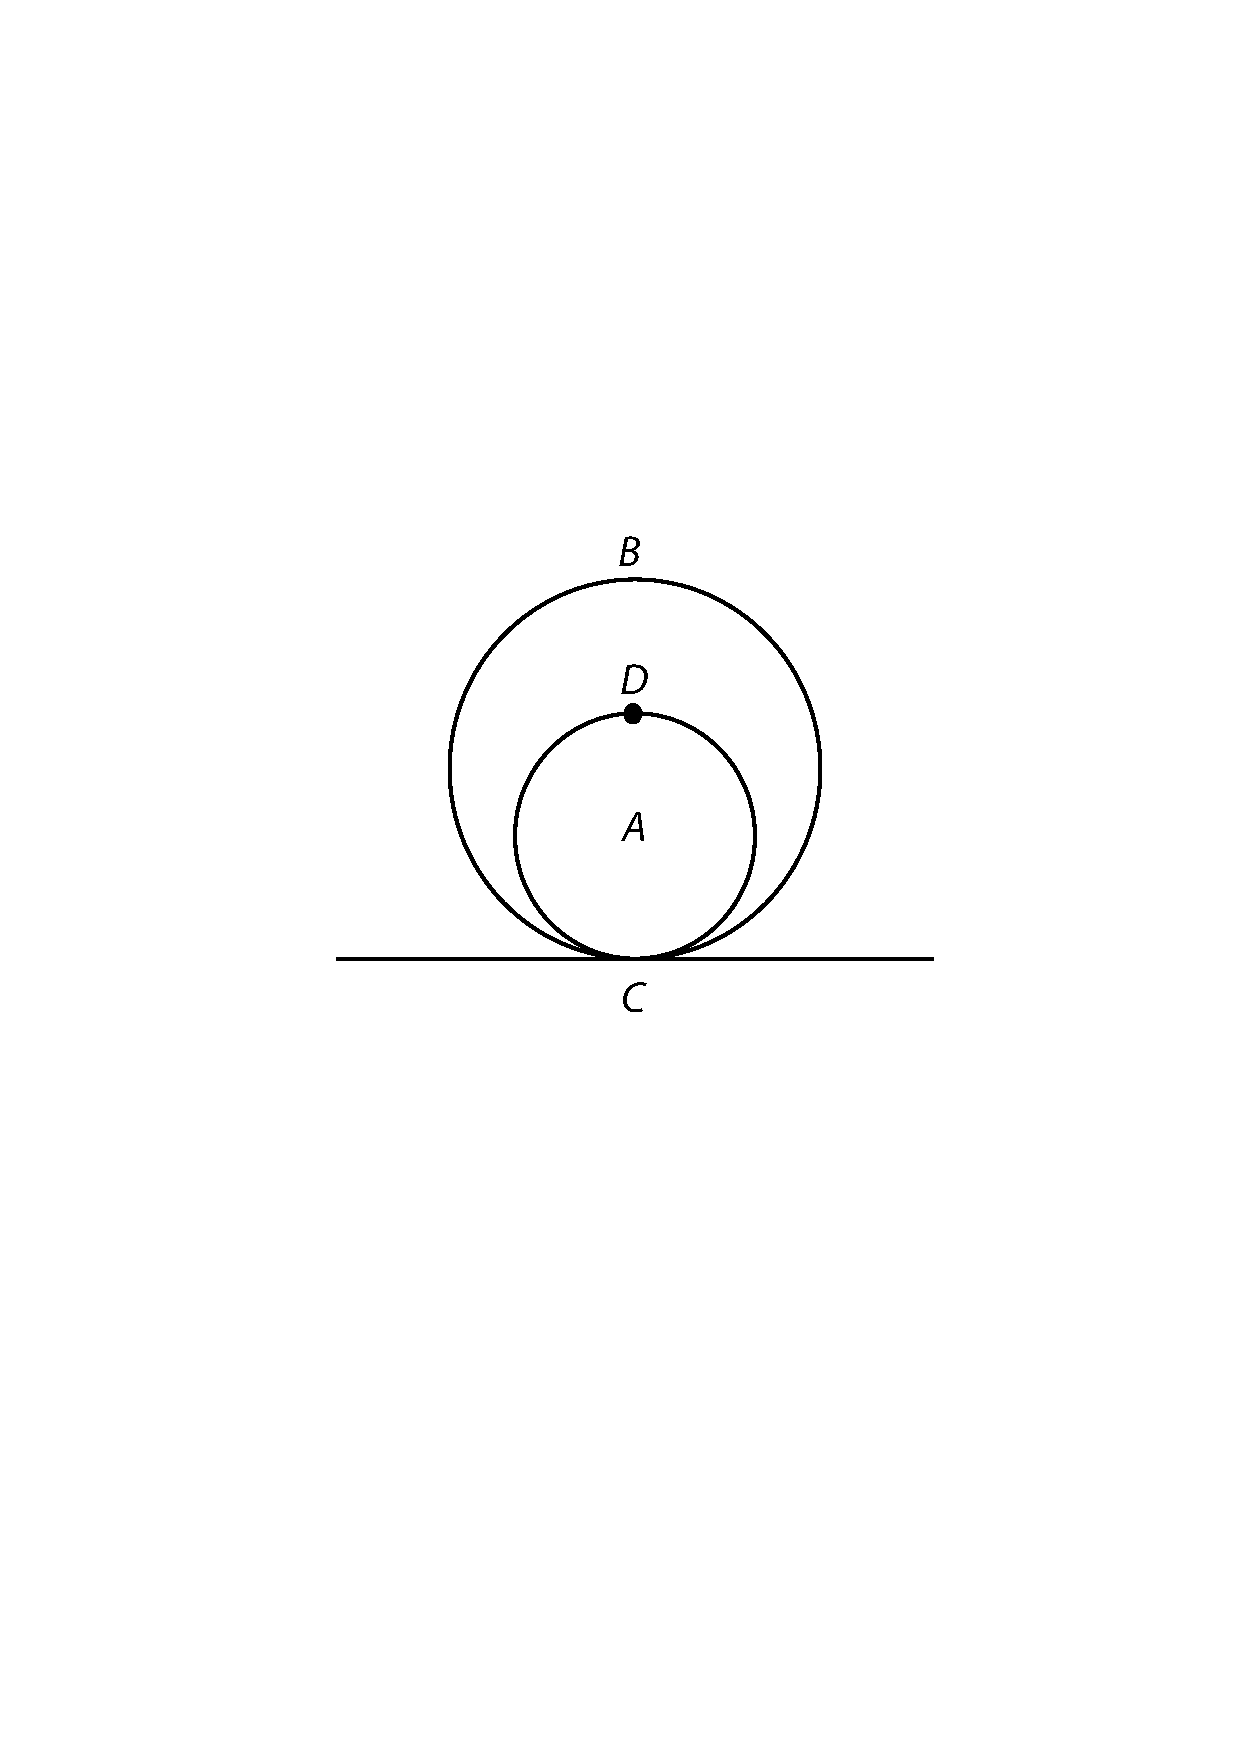
\includegraphics[trim = 0mm 0mm 0mm 0mm, clip, width=0.35\textwidth]{images/lh03705_009r-d2.pdf}\\
%    % \caption{Bildbeschreibung}
\noindent \centering [\textit{Fig. 10}] 
%\vspace{0,5em}
\pend
\vspace{1.5em}
\count\Cfootins=1100
\count\Bfootins=1100
\pstart
    Subjicere\setline{1} placet, solutionem difficultatis de duabus Rotis concentricis \edtext{ab Aristotele\protect\index{Namensregister}{\textso{Aristoteles}, 384-322 v. Chr.}}{\lemma{Aristotele}\Cfootnote{\cite{01002}\textit{Mech.} 24, 855a28-856a38.}} [motae]\edtext{}{\Bfootnote{motam\textit{\ \ L \"{a}ndert Hrsg.}}}, de qua \edtext{commentatores ejus mechanici,}{\lemma{commentatores ejus mechanici}\Cfootnote{Etwa \cite{01003}A. \textsc{Piccolomini}, \textit{In mechanicas quaestiones Aristotelis paraphrasis}, Rom 1547, cap. XXIX, S. 51r-54r; \cite{01004}G. \textsc{Biancani}, \textit{Aristotelis loca mathematica collecta et explicata}, Bologna 1615, Nr. 263, S.188-190; \cite{01005}B. \textsc{Baldi}, \textit{In mechanica Aristotelis problemata exercitationes}, Mainz 1621, quaestio XXIV, S. 146-150; \cite{01006}I. \textsc{de Guevara}, \textit{In Aristotelis mechanicas commentarii}, Rom 1627, quaestio XXIV, S. 205-224.}} sed et \edtext{Galilaeus\protect\index{Namensregister}{\textso{Galilei} (Galilaeus, Galileus), Galileo 1564-1642}}%
{\lemma{Galilaeus}\Cfootnote{\cite{00050}\cite{00048}\textit{Discorsi}, Leiden 1638, S.~21-26 (\textit{GO} VIII, S.~68-72).}} et \edtext{Tacquet\protect\index{Namensregister}{\textso{Tacquet}, Andre\'{e} SJ 1612-1660}}{\lemma{Tacquet}\Cfootnote{\cite{01007}A. \textsc{Tacquet}, \textit{Dissertatio physico-mathematica de circulorum volutionibus}, in \textit{Opera mathematica}, Antwerpen 1669, S. 143-168.}}, et Franciscus \edtext{Linus\protect\index{Namensregister}{\textso{Line} (Linus), Francis 1595-1675}}{\lemma{Linus}\Cfootnote{\cite{00072}F. \textsc{Line}, \textit{Tractatus de corporum inseparabilitate}, London 1661, cap. XXV-XXVII, S. 170-189.}} aliique acriter disputavere. Rota \textit{B} volvatur super plano \textit{AD}, in ea descriptus intelligatur
%%\begin{wrapfigure}{l}{0.5\textwidth}
%\begin{center}
%%\vspace{4mm}
%      \includegraphics[trim = 22mm 115mm 45mm 90mm, clip, width=0.53\textwidth]{images/lh03705_009r-d3.pdf}\\
%%\vspace{0.4em}
%\noindent [\textit{Fig. 11}] 
%\end{center}
%    % \caption{Bildbeschreibung}
%    %\end{wrapfigure} 
%\count\Cfootins=1500
%\count\Bfootins=1500
%\noindent 
circulus ei concentricus \textit{C}; \edtext{dum circulus}{\lemma{dum}\Bfootnote{\textit{(1)}\ rota \textit{(2)}\ circulus \textit{L}}} \textit{EB} provolvitur usque in \textit{D} ubi \textit{E}\hfill rursus\hfill ad\hfill planum\hfill revenisse\hfill ponatur[,]\hfill patet\hfill rectam\hfill \textit{ED}\hfill aequari\hfill circulo\hfill \textit{BE},\hfill eodem
\pend
\vspace{1em}
\pstart
\centering
\includegraphics[trim = 0mm 0mm 0mm 0mm, clip, width=0.58\textwidth]{images/lh03705_009r-d3.pdf}\\
\noindent \centering [\textit{Fig. 11}] 
\pend
\pstart
\noindent tempore et circulus \textit{FC} circuitum absolvet, et quando \textit{E} perveniet in \textit{D} tunc \textit{F} perveniet in \textit{G}. Jam circulus \textit{FC} continue \edtext{applicatur rectae}{\lemma{applicatur}\Bfootnote{\textit{(1)}\ lineae \textit{(2)}\ rectae \textit{L}}} \textit{FG}, ergo ejus circumferentia, rectae \textit{FG} aequalis, at recta \textit{FG} aequalis rectae \textit{ED}, et recta \textit{ED} circumferentiae \textit{EB}. Ergo circumferentia \textit{FC} circumferentiae \textit{EB}, quod est absurdum. Haec ut clarius intelligantur, filum circumligetur circumferentiae \textit{EB} quod iter provolvendo relinquet in plano. Rota \textit{FC} ponatur exire nonnihil ex \edtext{rota [\textit{EB}]}{\lemma{}\Bfootnote{\textit{CF}\textit{\ \ L \"{a}ndert Hrsg.}}}, et similiter in plano \edtext{substrato [\textit{FG}]}{\lemma{}\Bfootnote{\textit{CF}\textit{\ \ L \"{a}ndert Hrsg.}}} volvi, eique filum esse circumligatum, deinde circulorum loco polygona substituantur. Respondetur jam negando, polygonum interius plano \textit{FG} perfecte congruere[:] dum enim polygonum super centro \textit{E} erigitur tunc punctum \textit{F} surgit in \textit{H}, et punctum \textit{I} in \textit{K} ac proinde deseritur planum \textit{LG}.% \pend